\apendice{Especificación de Requisitos}

\section{Introducción}

Este anexo contendrá los objetivos de la aplicación y los requisitos que va a tener esta.
Consistirán en breves descripciones de todos los objetivos principales, como se subdividen en objetivos mas cortos para conseguir realizarlos y las funcionalidades implementadas.

Requisitos: Contendrá el que consiste el proyecto y las definiciones de los requisitos y objetivos.

\section{Objetivos generales}
\label{txt:objetivos}

Los objetivos que buscamos con este proyecto son:

\begin{itemize}
\item Construcción del prototipo de procesado de las imágenes:
Con este prototipo la funcionalidad buscada era, hacer las pruebas sobre el código, que mas adelante introduciríamos en la aplicación real, pero así podríamos ajustar los parámetros para que funcionase bien. También de esta forma estaríamos seguros que el proyecto es realizable.

\item Construcción de la aplicación: 
Una vez que tengamos el prototipo funcionando, tendríamos que construir una aplicación para ejecutar de una forma mas profesional que simplemente desde un notebook, esto es algo muy avanzado para un usuario sin experiencia, así facilitar la ejecución sin necesidad de depender del notebook.

\item  Construcción del prototipo para el modo automático:
Como hemos realizado el trabajo en tiempo, hemos optado por acoplar un modo de detección de bordes automatizado, para ver si eramos capaces de detectar los segmentos que detectaría un humano.
El problema de este modo es que algunos segmentos no son casi perceptibles por un humano por lo tanto los que estén mas marcados son los que podremos detectar.

\item Añadir el modo automático a la aplicación: 
Como hemos echo anteriormente con el modo de detección de las lineas pintadas. Esta vez también lo acoplaremos a nuestra aplicación, facilitando la ejecución y aplicación de este modo sobre imágenes que no estuvieran pintadas.
\end{itemize}



\section{Catalogo de requisitos}
El proyecto consiste en:
\begin{itemize}
	\item Construcción del prototipo de procesado de las imágenes.
		\begin{itemize}
			\item Lectura de imagen.
			\item Binarización para detectar las estrías pintadas.
			\item Procesado de la imagen binaria.
			\item Extracción de características.
			\item Procesado de las características.
		\end{itemize}
	\item Construcción de la aplicación.
		\begin{itemize}
			\item Lectura de imágenes y cargar en el panel.
			\item Construcción del panel de pestañas
			\item Construcción del modo de automático para lineas pintadas.
			\item Construcción del modo manual para corregir los errores o editar las lineas que hemos pintado.
			\item Construcción de la pestaña para el modo completamente automático.			
		\end{itemize}
	\item Construcción del prototipo para el modo automático.
		\begin{itemize}
			\item Lectura de la imagen.
			\item Equalizacion de la imagen para distribuir el histograma.
			\item Binarización para extraer bordes.
			\item Procesado de la imagen binaria para limpiar de ruido.
			\item Calculo de las características de la imagen.
			\item Procesado de características.		
		\end{itemize}
\end{itemize}


\section{Especificación de requisitos}
\begin{itemize}
	 
\item RF1: Construcción de la aplicación de forma gráfica.
	\begin{itemize}
		\item RF1.1: Construcción de los menús donde mostrar las opciones disponibles en la aplicación.
		\item RF1.2: Construcción del panel de pestañas donde estarán las opciones para los diferentes modos de la aplicación y sus funcionalidades
		\item RF1.3: Construcción del panel donde se mostrara la imagen junto con una barra de opciones con información de la imagen y botones de acciones sobre la imagen.
		\item RF1.4: Lectura de la imagen y cargar en el panel.
	\end{itemize}

\item RF2: Construcción del modo para calcular las estrías pintadas en las imágenes.
	\begin{itemize}
		\item RF2.1: Seleccionar el color de las estrías pintadas que queremos detectar.
		\item RF2.2: Seleccionar la orientación de la imagen, la longitud mínima que debe ignorar y el numero de repeticiones que quiere para calcular los segmentos.
		\item RF2.3: Pedir a la aplicación que use el algoritmo implementado para la detección de las estrías pintadas.			 
		\item RF2.4: Mostrar los segmentos que ha calculado con el algoritmo en el panel donde se muestra la imagen.
	\end{itemize}

\item RF3: Construcción del modo manual para corregir los errores o editar las lineas que hemos pintado.
	\begin{itemize}
		\item RF3.1: Pintar lineas sobre la imagen, pero solo sobre el cuadrado, para añadir nuevos segmentos.
		\item RF3.2: Añadir las lineas que ha calculado el algoritmo de detección de estrías pintadas.
		\item RF3.3: Borrar y limpiar la tabla de los segmentos obtenidos, que se corresponden con las estrías.
		\item RF3.4: Pintar, permitir mover y fijar el cuadrado donde queremos pintar las estrías manualmente.
		\item RF3.5: Guardar los segmentos y obtener las estadísticas y mediciones de todos los segmentos que ha calculado el algoritmo y se muestran en la tabla.			
	\end{itemize}
			 
\item RF4: Construcción del modo completamente automático para detectar las estrías en imágenes sin pintar.
	\begin{itemize}
		\item RF4.1: Seleccionar la orientación de la imagen y la longitud mínima que debe ignorar para calcular los segmentos. 
		\item RF4.2: Mandar calcular al algoritmo las estrías que contiene la imagen.
		\item RF4.3: Mostrar los segmentos que ha calculado con el algoritmo en el panel donde se muestra la imagen.					
		\item RF4.4: Pintar, permitir mover y fijar el cuadrado donde queremos quedarnos con las estrías.
	\end{itemize}
\end{itemize}					

\subsection{Diagrama de casos de uso}
El diagrama que contiene los caso de uso de nuestra aplicación esta contenido en la figura \ref{fig:diagramCasosUso}.	



\begin{figure}[h]
\centering
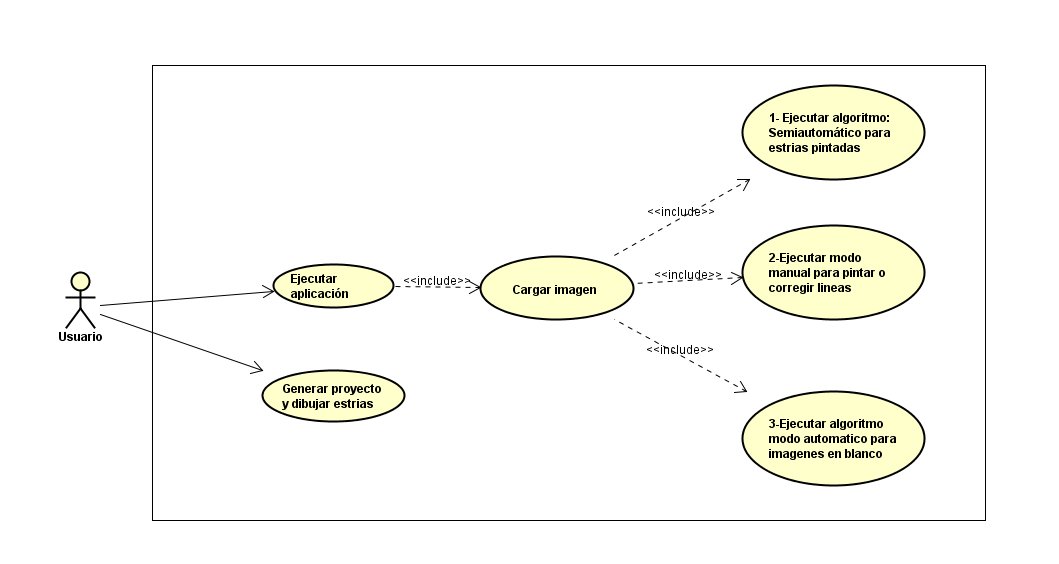
\includegraphics[width=.99\textwidth]{DiagramCasosUso}
\caption{Diagrama de casos de uso.}
\label{fig:diagramCasosUso}
\end{figure}
 
A partir del diagrama principal se han diseñado las siguientes tablas de los diagramas de casos de uso, se muestran en las siguientes figuras, \ref{tab:tablacaso1}, \ref{fig:tablacaso2}, \ref{fig:tablacaso3} y \ref{fig:tablacaso4}.

\begin{table}[]
\centering
\caption{Tabla del caso de uso 1}
\label{tab:tablacaso1}
\begin{tabular}{@{}
>{\columncolor[HTML]{FFFFFF}}l l@{}}
\toprule
\textbf{Caso de uso 1}   & Construcción Notebook interactivo de Júpiter,para imágenes pintadas.                                                                                                         \\ \midrule
\textbf{Versión}         & 1.0                                                                                                                                                                          \\ \midrule
\textbf{Autor}           & Ismael Tobar García                                                                                                                                                          \\ \midrule
\textbf{Requisitos}      & \begin{tabular}[c]{@{}l@{}}RF1\\   RF1.1\\   RF1.2\\   RF1.3\\   RF1.4\\   RF1.5\end{tabular}                                                                                \\ \midrule
\textbf{Descripción}     & \begin{tabular}[c]{@{}l@{}}El usuario podrá ejecutar el notebook interactivo para ver todo el proceso\\   paso a paso\end{tabular}                                           \\ \midrule
\textbf{Precondiciones}  & Tener una imagen con líneas pintadas.                                                                                                                                        \\ \midrule
\textbf{Acciones}        & \begin{tabular}[c]{@{}l@{}}1 Abrir notebook de Júpiter\\   2 Ir ejecutando paso a paso los bloques de código.\\   3 Se irán visualizando las partes ejecutadas.\end{tabular} \\ \midrule
\textbf{Postcondiciones} & Ninguna                                                                                                                                                                      \\ \midrule
\textbf{Excepciones}     & \begin{tabular}[c]{@{}l@{}}Si el usuario no ha especificado la ruta correcta a la imagen saltara\\   una excepción de que no existe el fichero.\end{tabular}                 \\ \midrule
\textbf{Importancia}     & Baja                                                                                                                                                                         \\ \bottomrule
\end{tabular}
\end{table}


			 


\begin{figure}[h]
\centering
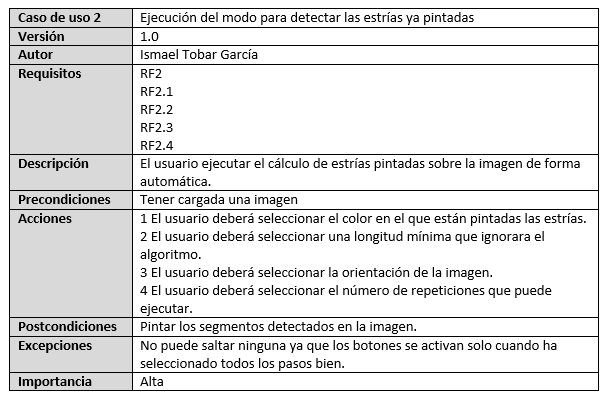
\includegraphics[width=.99\textwidth]{tablacaso2}
\caption{Tabla del caso de uso 2.}
\label{fig:tablacaso2}
\end{figure}

\begin{figure}[h]
\centering
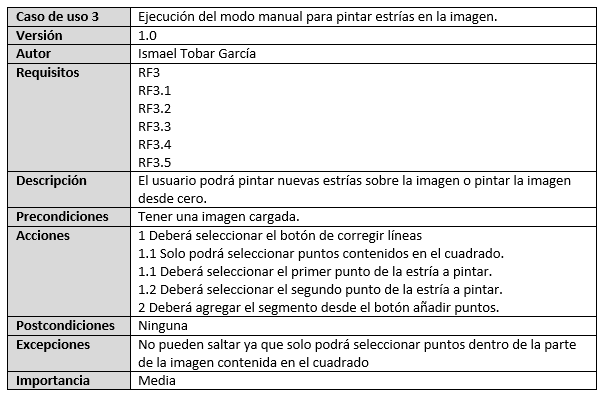
\includegraphics[width=.99\textwidth]{tablacaso3}
\caption{Tabla del caso de uso 3.}
\label{fig:tablacaso3}
\end{figure}

\begin{figure}[h]
\centering
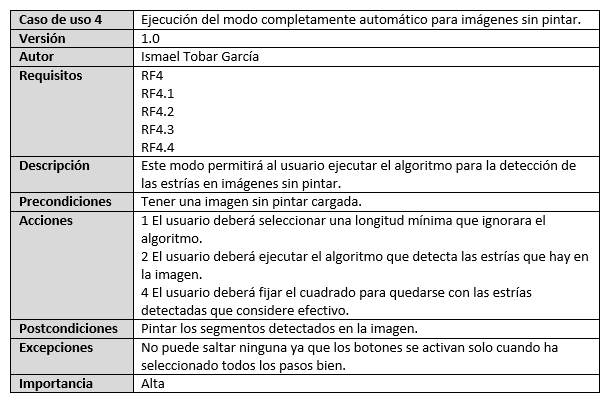
\includegraphics[width=.99\textwidth]{tablacaso4}
\caption{Tabla del caso de uso 4.}
\label{fig:tablacaso4}
\end{figure}
